\documentclass[conference]{IEEEtran}
\IEEEoverridecommandlockouts
% The preceding line is only needed to identify funding in the first footnote. If that is unneeded, please comment it out.
\usepackage{cite}
\usepackage{amsmath,amssymb,amsfonts}
\usepackage{graphicx}
\usepackage{textcomp}
\usepackage{xcolor}
\usepackage[ruled]{algorithm2e}
\def\BibTeX{{\rm B\kern-.05em{\sc i\kern-.025em b}\kern-.08em
    T\kern-.1667em\lower.7ex\hbox{E}\kern-.125emX}}
\begin{document}

\title{CECS: A Concurrent Entity Component System}

\author{\IEEEauthorblockN{Bramham}
\IEEEauthorblockA{\textit{College of Eng. and Computer Science} \\
\textit{University of Central Florida}\\
Orlando, Florida \\
connor.bramham@knights.ucf.edu}
\and
\IEEEauthorblockN{Vargas}
\IEEEauthorblockA{\textit{College of Eng. and Computer Science} \\
\textit{University of Central Florida}\\
Orlando, Florida \\
angel0615@knights.ucf.edu}
}

\maketitle

\begin{abstract}
The CECS is a project which implements concurrent programming concepts to meet the performance needs of modern simulated world applications. We discuss the correct program behavior of an Entity-Component-System, and the challenges associated with parallelizing this program behavior. We discuss the successes of previous entity-component-system projects, and opportunities we identified which could improve performance. We discuss how our ECS system compares to established work in the field. 
\end{abstract}

\begin{IEEEkeywords}
concurrent, entity-component-system, concurrency, archetypes, Rust language
\end{IEEEkeywords}

\section{Introduction}
An Entity-Component-System (ECS) is a software pattern used to simulate a model of some defined world. It is most often used in video games to simulate the game world. There are use cases for the ECS pattern outside of games as described in the "Review of Related Work" section. There is much debate over what an ECS actually is, but we will be using the model as described by Martin \cite{martin_2007}. In this model, there are three core concepts: the entity, the component, and the system. To demonstrate these concepts, examples will be given for practical use cases.

\subsection{Entity}
An entity is a "thing" within the world. They contain no data and have no logic. In essence, they are an identifier for some object, and because of this they are usually implemented simply as a unique integer identifier.

As an example of what an entity is, consider the game Flappy Bird. The bird and the pipes can be modeled as entities.

\subsection{Component}
A component is a piece of data that is associated with an entity. They are what give entities meaning. Components, like entities, have no logic. They are simply containers for data. An entity may have any number of components, including none at all (although the use cases for such entities is limited). Entities may also have many different kinds of components. Some implementations also allow for entities to have multiple instances of the same component type.


As an example, consider our previous example, Flappy Bird. As established before, the bird is an entity. To describe the bird, we may use the following components:
\begin{itemize}
\item A \verb|Controllable| component which acts as a flag to indicate that the bird can be controlled by the player.
\item A \verb|Renderable| component which describes how the bird should look on screen.
\item A \verb|Collider| component which enables collision detection with the pipes.
\item A \verb|RigidBody| component which allows the bird to fall following the laws of physics.
\item A \verb|Position| component which locates the bird in space.
\end{itemize}

We could describe the pipes using these components:
\begin{itemize}
\item A \verb|Renderable| component to show the pipe on screen.
\item A \verb|Collider| component which enables collision detection with the bird.
\item A \verb|Sliding| component to move the pipe from the right side of the screen to the left over time.
\item A \verb|Position| component which locates the pipe in space.
\end{itemize}

Notice that the pipes have a \verb|Sliding| component instead of a \verb|RigidBody| because they do not behave using the laws of physics. Additionally, since the pipes are not controlled by the player, they do not need a \verb|Controllable| component.

\subsection{System}
Systems are the logic that give entities behavior. They contain no data. A system mutates a subset of entities based on which components they have. The set of entities that a system operates on is typically called a query. The types of components requested in the query, including whether or not the component type will be mutated or only read, is called a filter.

For our Flappy Bird example, we might have the following systems:
\begin{itemize}
\item A \verb|Physics| system which operates on entities with both the \verb|RigidBody| and \verb|Position| components to apply physics computations. It may also operate on entities with both the \verb|Collider| and \verb|Position| components to resolve collisions.
\item A \verb|Renderer| system which operates on entities with both the \verb|Renderable| and \verb|Position| components to draw objects on the screen.
\item A \verb|PipeMover| system which operates on entities with both the \verb|Sliding| and \verb|Position| components to move them right to left.
\item A \verb|PlayerControl| system operates on entities with both the \verb|Controllable| and \verb|Position| components to allow the player to move them.
\end{itemize}

Notice that the \verb|Physics| system uses two queries. One is the set of entities with both the \verb|RigidBody| and \verb|Position| components. The other is the set of entities with the \verb|Collider| and \verb|Position| components.

\subsection{Review}
With only these three concepts it is clear that an ECS can adequately describe a real-world system. The role of the programmer is to describe the world they wish to model using these ideas. 

It should also be clear that this model differs heavily from traditional object-oriented programming paradigms. The ECS pattern prefers composition over inheritance and the separation of logic and data.

Beyond this brief overview, there are other concepts with appear often in the ECS ecosystem, including the idea of shared resources and events. The focus of this paper is on the idea of a dispatcher, which is the logic used to run the code associated with systems. Our goal was to create an algorithm for dispatchers which enables highly parallel execution of systems with as little overhead for the programmer using the ECS as possible. 

\section{Review of related work}
A good reference ECS, built with Rust, is the Specs project, maintained by the Amethyst organization. "Specs is close to the design of a classic ECS. Each component is stored in a Storage that contains a collection of like elements" \cite{sherratt_2020}. It was built to prioritizes flexibility and achieves a baseline performance relative to other ECS projects discussed here. 

The Amethyst organization built a successor to the Specs ECS, called Legion. "Legion aims to be a feature rich high performance Entity component system (ECS) library for Rust game projects" \cite{amethyst_github}. The biggest change between Specs and Legion is the use of a structure called an Archetype. This archetype structure improves entity search and filtering performance, "giving us contiguous runs of components which can be indexed together to access each entity" \cite{gillen_2020}. For a visual aid on ECS archetypes, refer to figure \ref{ECS Archetype} on page \pageref{ECS Archetype}. 

One of the most state of the art ECS projects in Rust is used by the Bevy game engine. Their project originally used a fork of an ECS called hecs, but switched over to a custom solution in version 0.5. Their new ECS uses a hybrid approach that combines the best of both a storage based and archetype based ECS.

The Concurrent Entity Component System takes inspiration from Legion's Archetype implementation, and attempts to improve upon existing dispatcher algorithms, increasing parallelization of work, and overall performance. The dispatcher algorithm can be thought of as a work scheduling algorithm, to coordinate thread usage of resources. 

The ECS systems from which our concurrent entity component system takes inspiration from are designed specifically for use in video game engines. However entity component systems have a much broader application than video games alone, and can be found in such applications as Geographical Wildlife Epidemiological Modeling \cite{https://doi.org/10.1111/gean.12258}, radar simulation \cite{radar_ECS} and graphical user interfaces \cite{10.1145/3331150}.

\section{Our Storage Model}

We took inspiration from Legion when deciding how to store component data. Our model, just like Legions, uses archetypes. An archetype can be thought of as an unordered set of component types that uniquely describes what components an entity has. Archetypes allocate buffers for each component type using a storage object that maintains a list of all buffers for a single type of component. Then, an archetype can store the components of entities that match with them into those buffers. In figure 1, you can see \verb|Archetype[A, B]| has two component types, \verb|A| and \verb|B|. There is a pointer into the storage objects for the allocated buffers. If we were to create an \verb|Entity 0| with component types \verb|A| and \verb|B|, the components for that entity would be stored in those storage buffers at the same index, \verb|i|. 

This archetype approach has a multitude of benefits. It makes it very easy for a system to access the entities with components they care about. A system can linearly iterate over each archetype and find the archetypes that contain all the component types the system operates on. Many archetype implementations often cache these look-ups to make them \verb|O(1)|. Additionally, iterating over all matching entities is extremely fast for modern hardware because the component data is stored in tightly packed linear buffers. This allows the CPU to make excellent usage of the cache and increases performance over storage based solutions which typically have random access patterns.

There are, however, trade offs that must be made. Typically, adding and removing components is slower than a storage based solution. This is because changing the component types of an entity changes its archetype, forcing it to be moved physically in memory from one location to another. Storage based solutions don't suffer from this problem because adding and removing components is usually a simple as changing a flag. 

However, because our work is based around massive parallelization we did not need to worry about fast addition and removal of components. Additionally, an archetype solution has a possible benefit for parallelization over storage based solutions that we will discuss later.
     
\begin{figure}
    \begin{center}
    \centerline{\includegraphics[scale=.43]{ECS_Diagrams.png}}
    \caption[test]{ECS Archetypes diagram}
    \label{ECS Archetype}
    \end{center}
\end{figure}

\section{Existing Parallelization Methods}

Before we took to creating our algorithm, we did an analysis of existing solutions. Following is a list of the algorithms we found and how they work.

\subsection{Fork Join}

This method was the simplest implementation, but also the one with least performance. In the fork join algorithm, you group together systems that can run together in parallel into stages. Then, you iterate over each stage, running all the systems in parallel and waiting for them all to finish before moving on to the next stage. You can see now that this algorithm gets its name from the behavior of parallelizing work by creating a "fork" where each "prong" is a system running in parallel, before "joining" all the prongs by waiting for each system to finish. 

Although it is easy to implement, this algorithm performs very poorly. Consider the example in figure 2. \verb|System 1| and \verb|System 3| form a stage and \verb|System 2| and \verb|System 4| form a stage. So, \verb|System 1| and \verb|System 3| will run in parallel first, finish, then move to the next stage. Consider, however, if \verb|System 3| were to finish before \verb|System 1|. If this were to occur, there would not longer be a data dependency over \verb|Component C| between the two stages. In other words, if \verb|System 3| finishes before \verb|System 1|, it should be possible to immediately begin running \verb|System 4|. With a fork join model, this is impossible because the stage must complete before running any other systems. This sort of stalling comes up a lot in real world systems, so the fork join model is often discarded for more efficient solutions.

\begin{figure}
    \begin{center}
    \centerline{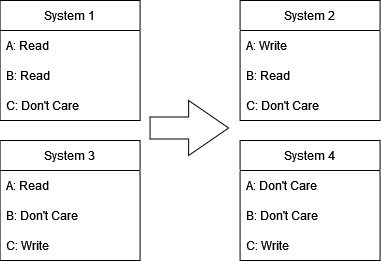
\includegraphics[scale=.6]{work_stealing.png}}
    \caption[test]{Fork Join Stalling}
    \label{ECS Archetype}
    \end{center}
\end{figure}

\subsection{Dynamic Load Balancing}

Dynamic load balancing is a technique used by Specs, and attempts to solve the issue of stalling in the fork join model. To do this, it adds a new concept called a group. A stage becomes composed of multiple groups, and groups are composed of multiple systems. The systems and groups are ordered in such a way that the systems of a group must run in serial because of data dependencies, but the groups of a stage may run in parallel. This, in and of itself, does not solve the stalling solution. To do so, at the end of dispatch, the scheduler analyzes the real time performance of each group. If it detects that one group is taking longer than another, it attempts to balance the load by moving systems around between groups. The optimization goal becomes trying to make each group take the same amount of real world time to finish. 

Although this does alleviate some of the issues of the fork join model, it does not completely solve the issue. This is because it can often by impossible to balance the load between two groups due to data dependencies. Additionally, systems can often have unpredictable performance. In one run a system might take a few milliseconds, but in another it might do no work at all. Because the load cannot be balanced until after dispatch when the timings become available, a system might be moved to another group when it shouldn't have been, leading to performance spikes.

\subsection{Realtime Topological Sorting}

The final parallel scheduling algorithm we analyzed was realtime topological sorting used by Bevy. This is similar to Kahn's algorithm, except it is performed every dispatch. So, at the start of dispatch, every system with no dependencies is send to a thread pool to be worked on. When a system completes, all of the systems dependent on the completed system are notified. When a system has been notified that all of its dependencies are complete, it can be sent to a thread pool. This process repeats until all systems have finished running.

This implementation performs the best out of the existing algorithms we discovered. However, we observed that there is still room for improvement. Consider the following scenario presented in figure 3.

\begin{figure}
    \begin{center}
    \centerline{\includegraphics[scale=.6]{TopoSort.png}}
    \caption[test]{Greedy Algorithm}
    \label{ECS Archetype}
    \end{center}
\end{figure}

Let us say that these are the only four systems in our dispatcher and they have no dependencies. So, they will all be told to run in parallel. However, they cannot all do so because \verb|System 1| has a data dependency between the other three systems. So, the question becomes "what selection of systems allows for the most to run in parallel?" Bevy solves this problem greedily and their output is shown in the upper part of figure 3. They iterate over each system, and take them as they can. So, Bevy sees \verb|System 1| and takes it because there is no existing conflict with any other systems that have been iterated over. Then, they iterate over all the other systems and don't take them because none of them are compatible with \verb|System 1|.

Clearly, this is not the best selection of systems. It is better to select \verb|System 2|,  \verb|System 3|, and  \verb|System 4| because it maximizes the number of systems running in parallel. This problem has yet to be tackled by an ECS in the Rust ecosystem, so our scheduler is designed specifically to avoid this problem.

\section{Our Algorithm}

The key insight for solving this problem was to view it in a different manner. In figure 4, we have the same set of systems and data dependencies as described in figure 3, but we represent them using a graph. Each system is represented by a vertex, and there is an edge between a vertex if the systems are able to run together in parallel. After seeing this, it became clear that we were attempting to find the maximum clique of a graph.

The maximum clique problem has thankfully already been solved (one of the most common solutions being the Bron-Kerbosch algorithm which we employed in our scheduler \cite{bron_kerbosch}). So, in essence, our scheduler is very similar to Bevy in that we perform a real-time topological sort to find what systems to run. Where our algorithm differs is that we select the optimal systems to run using the Bron-Kerbosch algorithm instead of selecting systems greedily. Algorithm 1 describes the scheduler in detail. Implementation details about caching are described in the performance section.

\begin{algorithm}
\SetKwInOut{Input}{input}
\Input{A set of systems $S$ to dispatch.}

$pending \gets $systems in $S$ with no dependencies\;
$running \gets \emptyset$\;
$finished \gets \emptyset$\;

\While{$finished \not= S$} {
    \tcp {Check if any systems are done running}
    \For{$r \in running$} {
        \If{$r$ is no longer running} {
            notify dependents and move to pending if they have no more dependencies\;
            $finished \gets finished \cup r$\;
        }
    }
    
    \tcp {Determine which systems to run}
    $ToRun \gets FromCache(running \cup pending)$\;
    
    \If{$ToRun = null$} {
        $ToRun \gets BronKerbosch(running \cup pending)$\;
        $IntoCache(running \cup pending, ToRun)$\;
    }
    
    \tcp {Send systems to a thread pool}
    \For{$sys \in ToRun$} {
        $running \gets running \cup sys$\;
        $pending \gets pending - sys$\;
        send sys to thread pool\;
    }
}

\caption{Scheduling Algorithm}
\end{algorithm}

\begin{figure}
    \begin{center}
    \centerline{\includegraphics[scale=.4]{Graph.png}}
    \caption[test]{System Graph}
    \label{ECS Archetype}
    \end{center}
\end{figure}

\section{Safety and Liveness}

The single invariant any scheduling algorithm must maintain in order to be safe is to only allow a single thread to mutate a resource at a time. Taking inspiration from the Rust language which we used to implement our scheduler, you can have as many immutable references to something as you want, but if you ever have a mutable reference, it must be the only reference. By maintaining this invariant, we can guarantee safety.

The shared data being accessed in an ECS is component data. So, our algorithm must guarantee that any two systems running in parallel maintain the safety invariant. This is done using a language feature in Rust called an associated type. When creating a new system, we enforce that the system must define what component types it will operate on and whether it will need mutable or immutable access to those component types. This is represented as a tuple, and is a type described at compile time. It is similar to an archetype, except for the additional information about mutable or immutable access requirements. The scheduler can use this information to determine if any two systems may run in parallel together, guaranteeing safety for our scheduler.

Our algorithm is lock-free. We guarantee that at least one thread is performing work because we never submit work to the thread pool unless we guarantee it can run with existing threads. So, once a thread receives work it knows it can run without waiting. However, it is virtually impossible to achieve wait freedom unless you also guarantee that each system is wait free. 

\section{Performance}

While implementing our scheduler, we discovered a few surprising things that led to poor performance. Here, we will list these challenges and how we overcame them. These are listed in order of implementation, so performance improvements are relative to the previous optimization.

\subsection{Bron-Kerbosch}

The biggest performance bottle-neck turned out to be the Bron-Kerbosch algorithm. As it turns out, the algorithm is in the class NP-complete, which means all algorithms that solve the problem run in exponential time. This was a issue for us because this algorithm may be run multiple times every dispatch, and often a dispatch must complete in less than a few milliseconds in order to maintain real-time performance. 

Our solution to this issue is to use caching. We observed that, when a set of systems has been run through the algorithm, it's output does not need to be recomputed. Instead, we can hold onto the result and reference next time we encounter the same set of systems. This reduced our run times by a factor of ten, and was the most significant change that allowed us to get maximum performance.

\subsection{Memory Allocation}

The next biggest performance bottleneck was memory allocation. Every dispatch, we maintain a list of pending, complete, and finished systems in hash sets. These lists must be allocated at runtime, which greatly reduced performance. Our simple fix used caching. Instead of reallocating these hash sets every dispatch, we reuse them between dispatches, and simply clear them at the start. This gave us a speed boost of three times.

\subsection{Thread Pool Contention}

Our initial implementation used a single wait free queue to signal to the main thread when a system finished running. When a system finished running, it would send back to the main thread a unique identifier. Then the main thread would then iterate over all the systems that finished running by pulling their identifiers out of the queue. The problem that arose was from contention in the queue.

Although the channels are designed to minimize contention, it is still possible to get reduced performance when threads submit to the same channel rapidly. Our solution was to give each system it's own flag that signals when it is complete. The main  thread then keeps track of running systems on its own and checks each of the flags separately. This modification meant that there was no longer any contention on the channels. This gave us a speed improvement of approximately two times.

\subsection{System Sets}

With large numbers of systems, the number of permutations of systems in the cache for Bron-Kerbosch can reach into the hundreds. To store systems, we initially used heap allocated hash sets of unique identifiers for systems. This was poor for both memory and performance because we not only had to heap allocate for each set of systems, but the caching algorithm was forced to hash a hash set, which is very slow.

To resolve this, we chose to represent systems using bit-sets. Each bit in the bit-set corresponds to a single system. If the bit is 1, it means the system is in the set and if it's 0 it isn't in the set. This significantly sped up hashing because we were merely hashing a few integers. It also sped up the Bron-Kerbosch algorithm because certain set operations could be performed using bit-wise operations. We saw performance improvements of up to three times.

\subsection{Benchmarking}

We chose to only benchmark our algorithm against Bevy's scheduler for the following reasons.

\begin{itemize}
\item Our preliminary benchmarks showed that Bevy outperformed Specs and Legion, so if we perform better than Bevy we perform better than them as well.
\item Due to Rust lacking a language feature called variadic generics, it is impossible to implement type based component access descriptions for systems for arbitrary numbers of components. This forces Rust ECS implementations to pick an upper limit on the number of types of components a system can access at a time. Legion only allows 8 component types, which makes certain tests impossible to perform because we need to access more.
\item Bevy's implementation is extremely similar to ours except for the system selection during tie breaking.
\end{itemize}

Our test system used a stock AMD Ryzen 2500U, with 4 physical cores and 8 logical threads. We compared our algorithms over different iteration counts and different thread counts. Each set of iterations were performed three times and then averaged. You can see the results of our benchmark on different systems graphs in figures 5, 7, 9, and 11 with respective system graphs in figures 6, 8, 10, and 12. These figures are located in Appendix A.

Benchmark one was designed to be a real world test case. The dependency relationship here is used by a real game made as a student project by one of our researchers in a previous semester. It has a complex dependency relationship which our algorithm should solve easily, whereas Bevy will struggle because the greedy solution here is not optimal.

Benchmark two was designed to be a near-best case scenario for our implementation. Here, we have three components of the system graph with differing sizes. The systems are added in such an order that Bevy will choose poorly each time, while our implementation will detect the maximum cliques and select them easily. This is because Bevy selects systems linearly. If we were to reverse the order of the systems (i.e. making the $K_5$ graph come first in the ordering) Bevy would select optimally.

Benchmark three was generated randomly and acts as a generic test case for both systems. However, it does have a complex dependency relationship which we hypothesized would be optimal for our implementation.

Benchmark four was designed to be a best case scenario for Bevy. It is the maximally connected graph $K_6$ which means any selection of systems in any order will produce an optimal selection. We hypothesized that Bevy would outperform us in this benchmark.

\section{Discussion and Conclusion}

It is clear that our solution performs significantly better than the state of the art in the Rust ecosystem. By choosing the optimum selection of systems instead of choosing them greedily, we outperform other implementations, even in their best case scenarios. Benchmark four demonstrates just how much performance we can gain by selecting optimally. In the one-million iteration run, we performed over six times faster than Bevy. 

It's also worth noting that we have significantly better performance even in the best case for Bevy. Benchmark four demonstrates a fully connected set of systems which is optimal for the greedy solution. However, our algorithm still outperforms Bevy. Our original hypothesis here was proven incorrect because of this. Our revised hypothesis is that Bevy is forced to perform the greedy algorithm every dispatch. This means they need to constantly keep track of what resources are being read from and written to. However, our algorithm only needs to run Bron-Kerbosch once, and then it can refer to the cache for the system selection. This means that Bevy is performing an \verb|O(N)| operation every dispatch, whereas our implementation only needs to perform the Bron-Kerbosch algorithm once and then it can refer to the cache in \verb|O(1)| time.

Benchmark one shows an interesting property of our scheduler. The one-hundred-thousand iteration run performed slower than Bevy, but the one-million iteration run performed faster. This is due to the algorithm still needing to build up the cache. In the shorter run, the cache did not have enough time to be built, but in the longer one it did. For applications such as gaming, this is not a concern because the dispatcher might have hours to build it's cache.

There are other possible optimizations that could be made to the scheduler. One optimization that was discussed involved a tie-breaking scenario due to Bron-Kerbosch. The Bron-Kerbosch algorithm produces a list of sets of systems which represent maximal cliques. The maximum clique is selected by taking the largest of the maximal cliques. However, it is possible that two sets of maximal cliques might have the same number of systems. In this case, a tie needs to be broken, but the question becomes "how do we break the tie optimally?" It might be possible to combine aspects of Specs dynamic load balancing to keep track of the runtime of systems so you could select the set that maximizes throughput. However, more research needs to done to determine an algorithm for such a scheduler.

Additionally, there are other aspects of an ECS that could benefit from parallelization. One such aspect is entity iteration. Systems frequently need to query the world for entities that match certain archetypes. When a query is made, the component buckets that make up each compatible archetype are linked together. However, these linked component buckets are independent of each other. It is possible that one could iterate over the entities of each bucket in parallel to see significant performance gains when archetypes are highly fragmented. Furthermore, entity creation and destruction along with component addition and removal at runtime are common operations. It is desirable to have these operations become atomic so they can be performed simultaneously from multiple threads. Existing solutions solve this problem by deferring these operations to the beginning of dispatch, but we hypothesize that performance gains could be found by allowing these operations to be performed simultaneously.

We'd like to thank Dr. Dechev for aiding in our understanding of parallel programming and James Voor for his aid on the research paper.

\bibliographystyle{plain} 
\bibliography{refs}

\section{Appendix A}

\begin{figure}[!htb]
    \begin{center}
    
    \begin{tabular}{||c c c||} 
    \hline
    Num. Iterations & CECS & Bevy  \\ [0.5ex] 
    \hline\hline
    1,000 & 13 ms & 19 ms \\ 
    \hline
    100,000 & 1,765 ms & 1,514 ms \\
    \hline
    1,000,000 & 9,393 ms & 15,153 ms \\
    \hline
    \end{tabular}
    
    \caption[test]{Benchmark 1 Data}
    \label{Benchmark 1 Data}
    \end{center}
\end{figure}

\begin{figure}[!htb]
    \begin{center}
    \centerline{\includegraphics[scale=.6]{BM4.png}}
    \caption[test]{Benchmark 1 System Graph}
    \label{Benchmark 1 System Graph}
    \end{center}
\end{figure}

\begin{figure}[!htb]
    \begin{center}
    
    \begin{tabular}{||c c c||} 
    \hline
    Num. Iterations & CECS & Bevy  \\ [0.5ex] 
    \hline\hline
    1,000 & 10 ms & 21 ms \\ 
    \hline
    100,000 & 933 ms & 2,134 ms \\
    \hline
    1,000,000 & 9,362 ms & 27,569 ms \\
    \hline
    \end{tabular}
    
    \caption[test]{Benchmark 2 Data}
    \label{Benchmark 2 Data}
    \end{center}
\end{figure}

\begin{figure}[!htb]
    \begin{center}
    \centerline{\includegraphics[scale=.5]{BM1.png}}
    \caption[test]{Benchmark 2 System Graph}
    \label{Benchmark 2 System Graph}
    \end{center}
\end{figure}

\begin{figure}[!htb]
    \begin{center}
    
    \begin{tabular}{||c c c||} 
    \hline
    Num. Iterations & CECS & Bevy  \\ [0.5ex] 
    \hline\hline
    1,000 & 10 ms & 33 ms \\ 
    \hline
    100,000 & 930 ms & 2,616 ms \\
    \hline
    1,000,000 & 9,522 ms & 17,225 ms \\
    \hline
    \end{tabular}
    
    \caption[test]{Benchmark 3 Data}
    \label{Benchmark 3 Data}
    \end{center}
\end{figure}

\begin{figure}[!htb]
    \begin{center}
    \centerline{\includegraphics[scale=.5]{BM2.png}}
    \caption[test]{Benchmark 3 System Graph}
    \label{Benchmark 3 System Graph}
    \end{center}
\end{figure}

\begin{figure}[!htb]
    \begin{center}
    
    \begin{tabular}{||c c c||} 
    \hline
    Num. Iterations & CECS & Bevy  \\ [0.5ex] 
    \hline\hline
    1,000 & 4 ms & 20 ms \\ 
    \hline
    100,000 & 464 ms & 2,451 ms \\
    \hline
    1,000,000 & 4,788 ms & 29,011 ms \\
    \hline
    \end{tabular}
    
    \caption[test]{Benchmark 4 Data}
    \label{Benchmark 4 Data}
    \end{center}
\end{figure}

\begin{figure}[!htb]
    \begin{center}
    \centerline{\includegraphics[scale=.5]{BM3.png}}
    \caption[test]{Benchmark 4 System Graph}
    \label{Benchmark 4 System Graph}
    \end{center}
\end{figure}

\end{document}